This chapter focuses on a comprehensive literature review encompassing four key subjects: Colorectal Cancer (CRC), Operations Research through Process Mining, Process Mining in healthcare, and Simulation in healthcare. Each of these subjects holds significant relevance for the thesis, playing crucial roles in understanding and improving healthcare processes in the context of CRC diagnosis and treatment.

Colorectal cancer stands as the central focus, representing the medical condition under examination. In an Operations Research context, Process Mining offers a direct path to reveal how a process functions and behaves. Process Mining in healthcare serves as a powerful analytical tool to explore the intricate pathways involved in CRC care. Similarly, Simulation in healthcare offers a dynamic platform for modeling and evaluating various scenarios, providing insights into the potential impacts of process optimizations and interventions in CRC management. This thesis aims to establish a solid foundation of knowledge and insights to inform the subsequent methodological approach through a comprehensive review

\section{Colorectal Cancer}

It is important to mention that this thesis focuses on colorectal cancer from a perspective previously involved in operations research. Therefore, certain advances specifically in the medical field are omitted from the state of the art.

Various studies have been conducted on the diagnosis and treatment of this disease from an epidemiological \cite{marley_epidemiology_2016} and operational perspective \cite{lieberman_screening_2009, vega_colorectal_2015, wolpin_systemic_2008}. All cancers tend to increase in complexity over time, so early diagnosis is crucial to increase the chances of success and reduce treatment costs \cite{kakushadze_estimating_2017}.

Regarding CRC, the confirmation method is the colonoscopy exam. This procedure is effective but costly in terms of both monetary and healthcare personnel resources. Therefore, in most healthcare systems, it is considered a scarce resource that must be used judiciously \cite{kolligs_diagnostics_2016}. There is also variability in the detection capacity of CRC depending on the expertise of the personnel performing the exam \cite{okada_international_2016}.

There is a trend to recommend the use of screening methods to improve patient prognosis \cite{bretthauer_colorectal_2011}. According to \citeA{lansdorp-vogelaar_effect_2009}, almost all recommended screening methods save money for healthcare systems, especially the use of fecal occult blood tests due to their cost-effectiveness \cite{winawer_colorectal_2007}. There are different types of these tests, with fecal immunochemical testing (FIT) showing the best performance in terms of sensitivity and specificity \cite{zhu_comparison_2010}. Additionally, there are several fecal immunochemical tests with similar performance parameters \cite{lee_accuracy_2014}. It is important to mention that by reducing the cutoff value of this test, a greater number of colonoscopies is required, so the optimal value depends on the system's capacity to perform this procedure.

\begin{tcolorbox}[title=Sensitivity and Specificity of a Test, width=\textwidth, colback=white, colframe=black, fonttitle=\bfseries, boxrule=0.5mm]

The description of these tests metrics according to \citeA{trevethan_sensitivity_2017} are:

\begin{center}
    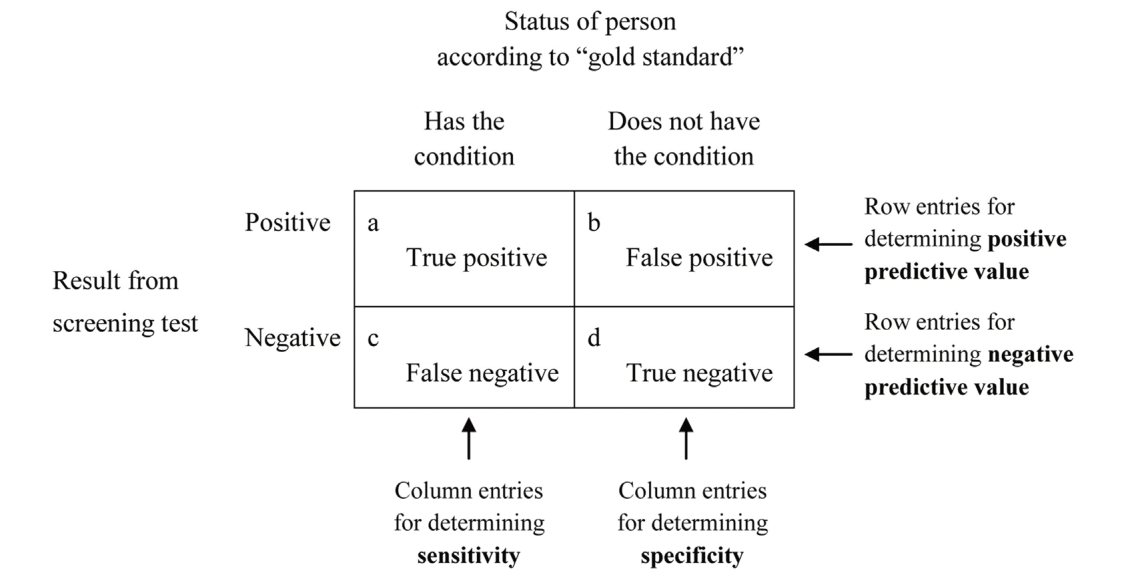
\includegraphics[width=1\textwidth]{images/2.literature_review/sensitivity_and_specificity.png}
    \captionof{figure}{Diagram demonstrating the basis for deriving sensitivity, specificity, and positive and negative predictive values\textsuperscript{1}}
    \label{fig:sensitivity_and_specificity}
\end{center}

\bigskip
        The sensitivity of a test refers to its ability to accurately detect true positives, meaning it correctly identifies all individuals who have a condition. That means that sensitivity is based solely on the cells labeled \textbf{a} and \textbf{c} in Figure \ref{fig:sensitivity_and_specificity}.\\
        Contrariwise, the specificity of a test measures its ability to accurately detect true negatives, meaning it correctly identifies individuals who do not have a condition. That means that specificity is based on the cells labeled \textbf{b} and \textbf{d} in Figure \ref{fig:sensitivity_and_specificity}.

\end{tcolorbox}

\footnotetext[1]{From \textit{Sensitivity, Specificity, and Predictive Values: Foundations, Pliabilities, and Pitfalls in Research and Practice} by R. Treevethan, 2017, Front in Public Health, 5, p. 307. Creative Commons Attribution License }

The research conducted by \citeA{navarro_colorectal_2017} demonstrates the extensive adoption of CRC screening strategies globally, encompassing most European countries, Canada, specific regions in North and South America, Asia, and Oceania. These initiatives typically employ either the FIT or fecal occult blood test (FOBT) in conjunction with colonoscopies to facilitate early detection of CRC within their respective populations. The study highlights varying participation rates, with notable examples such as the Netherlands boasting a 68.2\% participation rate, providing valuable insights into successful approaches. On the other hand, instances like Canada, with participation rates as low as 16\%, underscore potential practices to be avoided.

\section{Briging the Gap: Operations Research and Process Mining}

Operations Management, for many years, has developed tools for process analysis, which are commonly found in any reference of the discipline \cite{rama_murthy_operations_2007}. However, in recent times, the digitization of many processes has made a large amount of data available regarding the processes and the flows of activities within them. The analysis of this data using sophisticated tools, such as those derived from Machine Learning topics, taking into account the underlying processes, has led to the methodology called Process Mining, which has been very successful in the analysis and improvement of complex processes \cite{van_der_aalst_process_2004}.

\section{Process Mining}

Process Mining, as a methodological approach, has gained prominence in various industries for its capability to extract valuable insights from event data. For example, it has been used in education to help predict the success of students in massive online courses with high accuracy \cite{umer_predicting_2017}, and in product design to enhance medical machines that require operator interaction \cite{reindler_siemens_2020}.

In the healthcare sector, where process complexity often impedes efficient care delivery, there are numerous instances where process mining holds the potential to uncover hidden patterns, identify bottlenecks, and enhance overall service quality \cite{rojas_process_2016}. Various authors advocate that this tool allows for modeling processes and studying them from different perspectives, including visual representations, activity durations, time between activities, variability, expected behavior versus actual behavior, and many others \cite{bozkaya_process_2009}.

When applied to CRC care, Process Mining serves as a lens through which the complexities of detection, confirmation, categorization, and treatment processes can be systematically analyzed.

\section{Simulation}

Simulation holds significant importance within in the realm of Operations Research \cite{de_paula_ferreira_simulation_2020}, serving as a powerful tool for analyzing complex systems and making informed decisions. In Operations Research, Simulation enables researchers and practitioners to model intricate processes, test various scenarios, and evaluate the impact of different strategies without the need for real-world experimentation. According to Dr. Nelson in \cite{fu_simulation_2014}, Simulation is typically used for three reasons: feasibility (“We have a plan, will it work?”); sensitivity (“We’re not really sure about everything, so how much does it matter?”); and optimization (“What are the good options and how good are they?”). Simulation Optimization is a well known topic in the Simulation community, addressing the problem of designing complex systems by finding the best settings of design variables.

Similarly, in healthcare, Simulation plays a crucial role in improving the delivery of care, enhancing patient outcomes, and optimizing resource allocation \cite{jun_application_1999}. Healthcare systems are inherently complex, involving a multitude of interconnected factors such as patient flow, resource utilization, staffing levels, and treatment protocols. Simulation in healthcare serves primarily four purposes: health and care systems operation (HCSO), disease progression modeling (DPM), screening modeling (SM), and health behavior modeling (HBM), with the most prevalent being HCSO, followed by DPM, SM, and HBM, respectively \cite{zhang_application_2018}. From predicting patient wait times in emergency departments to optimizing operating room schedules and evaluating the efficacy of new treatment protocols, Simulation offers invaluable insights that can inform decision-making, improve efficiency, and ultimately enhance patient care.

Screening simulations are essential tools for evaluating the potential implementation of screening programs, assessing their impact on prognosis, cost-effectiveness, and implementation feasibility. These simulations find applications in various healthcare areas, including the detection of diseases like diabetic retinopathy \cite{davies_evaluation_2002} and numerous types of cancers \cite{bespalov_cancer_2021}.

Prior to the twenty-first century, computer simulations were not seen as providing evidence definitive enough to shape screening recommendations \cite{phillips_screening_2020}. A major turning point for the CRC screening simulations came when three independent simulation models were developed for CRC: the MIcrosimulation SCreening Analysis Colorectal Cancer Model (MISCAN-Colon)\cite{loeve_miscan-colon_1999}, the Simulation Model of Colorectal Cancer (SimCRC)\cite{knudsen_rescreening_2012}, and the Colorectal Cancer Simulated Population model for Incidence and Natural history (CRC-SPIN)\cite{rutter_bayesian_2009}. The MISCAN-Colon model, introduced in 1999, has served as a foundational framework for numerous subsequent models developed in the following years \cite{smith_simulation_2020}.